\documentclass[]{elsarticle} %review=doublespace preprint=single 5p=2 column
%%% Begin My package additions %%%%%%%%%%%%%%%%%%%
\usepackage[hyphens]{url}
\usepackage{lineno} % add
\providecommand{\tightlist}{%
  \setlength{\itemsep}{0pt}\setlength{\parskip}{0pt}}

\bibliographystyle{elsarticle-harv}
\biboptions{sort&compress} % For natbib
\usepackage{graphicx}
\usepackage{booktabs} % book-quality tables
%% Redefines the elsarticle footer
%\makeatletter
%\def\ps@pprintTitle{%
% \let\@oddhead\@empty
% \let\@evenhead\@empty
% \def\@oddfoot{\it \hfill\today}%
% \let\@evenfoot\@oddfoot}
%\makeatother

% A modified page layout
\textwidth 6.75in
\oddsidemargin -0.15in
\evensidemargin -0.15in
\textheight 9in
\topmargin -0.5in
%%%%%%%%%%%%%%%% end my additions to header

\usepackage[T1]{fontenc}
\usepackage{lmodern}
\usepackage{amssymb,amsmath}
\usepackage{ifxetex,ifluatex}
\usepackage{fixltx2e} % provides \textsubscript
% use upquote if available, for straight quotes in verbatim environments
\IfFileExists{upquote.sty}{\usepackage{upquote}}{}
\ifnum 0\ifxetex 1\fi\ifluatex 1\fi=0 % if pdftex
  \usepackage[utf8]{inputenc}
\else % if luatex or xelatex
  \usepackage{fontspec}
  \ifxetex
    \usepackage{xltxtra,xunicode}
  \fi
  \defaultfontfeatures{Mapping=tex-text,Scale=MatchLowercase}
  \newcommand{\euro}{€}
\fi
% use microtype if available
\IfFileExists{microtype.sty}{\usepackage{microtype}}{}
\usepackage[left=2.5cm,right=2.5cm,top=2.5cm,bottom=2.5cm]{geometry}
\usepackage{longtable}
\usepackage{graphicx}
% We will generate all images so they have a width \maxwidth. This means
% that they will get their normal width if they fit onto the page, but
% are scaled down if they would overflow the margins.
\makeatletter
\def\maxwidth{\ifdim\Gin@nat@width>\linewidth\linewidth
\else\Gin@nat@width\fi}
\makeatother
\let\Oldincludegraphics\includegraphics
\renewcommand{\includegraphics}[1]{\Oldincludegraphics[width=\maxwidth]{#1}}
\ifxetex
  \usepackage[setpagesize=false, % page size defined by xetex
              unicode=false, % unicode breaks when used with xetex
              xetex]{hyperref}
\else
  \usepackage[unicode=true]{hyperref}
\fi
\hypersetup{breaklinks=true,
            bookmarks=true,
            pdfauthor={},
            pdftitle={Journal Paper Template : An RMarkdown template for writing a journal article},
            colorlinks=true,
            urlcolor=blue,
            linkcolor=magenta,
            pdfborder={0 0 0}}
\urlstyle{same}  % don't use monospace font for urls
\setlength{\parindent}{0pt}
\setlength{\parskip}{6pt plus 2pt minus 1pt}
\setlength{\emergencystretch}{3em}  % prevent overfull lines
\setcounter{secnumdepth}{5}
\usepackage{setspace}
\doublespacing
% Pandoc toggle for numbering sections (defaults to be off)
% Pandoc header
\usepackage{setspace}
\doublespacing


\usepackage[nomarkers]{endfloat}

\begin{document}
\begin{frontmatter}

  \title{Journal Paper Template : An RMarkdown template for writing a journal
article}
    \author[CBE]{Firstname1 Lastname1\corref{c1}}
   \ead{cbe.researcher@berkeley.edu} 
   \cortext[c1]{Corresponding Author}
    \author[Manufacturer]{Firstname2 Lastname2}
  
  
    \author[Visiting]{Firstname3 Lastname3}
  
  
    \author[CBE]{Firstname4 Lastname4}
  
  
    \author[Consultant]{Firstname5 Lastname5}
  
  
      \address[CBE]{Center for the Built Environment, UC Berkeley, 390 Wurster Hall,
Berkeley, CA, 94720, USA}
    \address[Manufacturer]{Collaborating Manufacturer, 1234 Innovation Dr, Lexington, KY 12345, USA}
    \address[Visiting]{Dept. of Environment Science and Engineering, Daxue University, 123
Xuexiao Road, Tianjin, 123456, China}
    \address[Consultant]{Consulting company, 123 54th St, Oakland, CA, 12345, USA}
  
  \begin{abstract}
  Abstract text goes here. This template was craeted by Dana Miller is
  adapted from code and text in the submitted manuscript ``Ceiling fans -
  Predicting indoor air speeds based on full scale laboratory
  measurements'' by Paul Raftery et al. All data and analysis code in this
  paper is avalible at \url{https://github.com/dmgt/draft-template}.
  \end{abstract}
  
 \end{frontmatter}

Keywords:\\
Ceiling fan; Air speed distribution; Full-scale laboratory testing;
Rotational speed; Fan diameter; Fan direction

\pagebreak

\textbf{Highlights:}

\begin{itemize}
\tightlist
\item
  Hightlight 1
\item
  Highlight 2
\item
  Highlight 3
\item
  Highlight 4
\item
  Highlight 5
\end{itemize}

\textbf{Graphical Abstract}\\
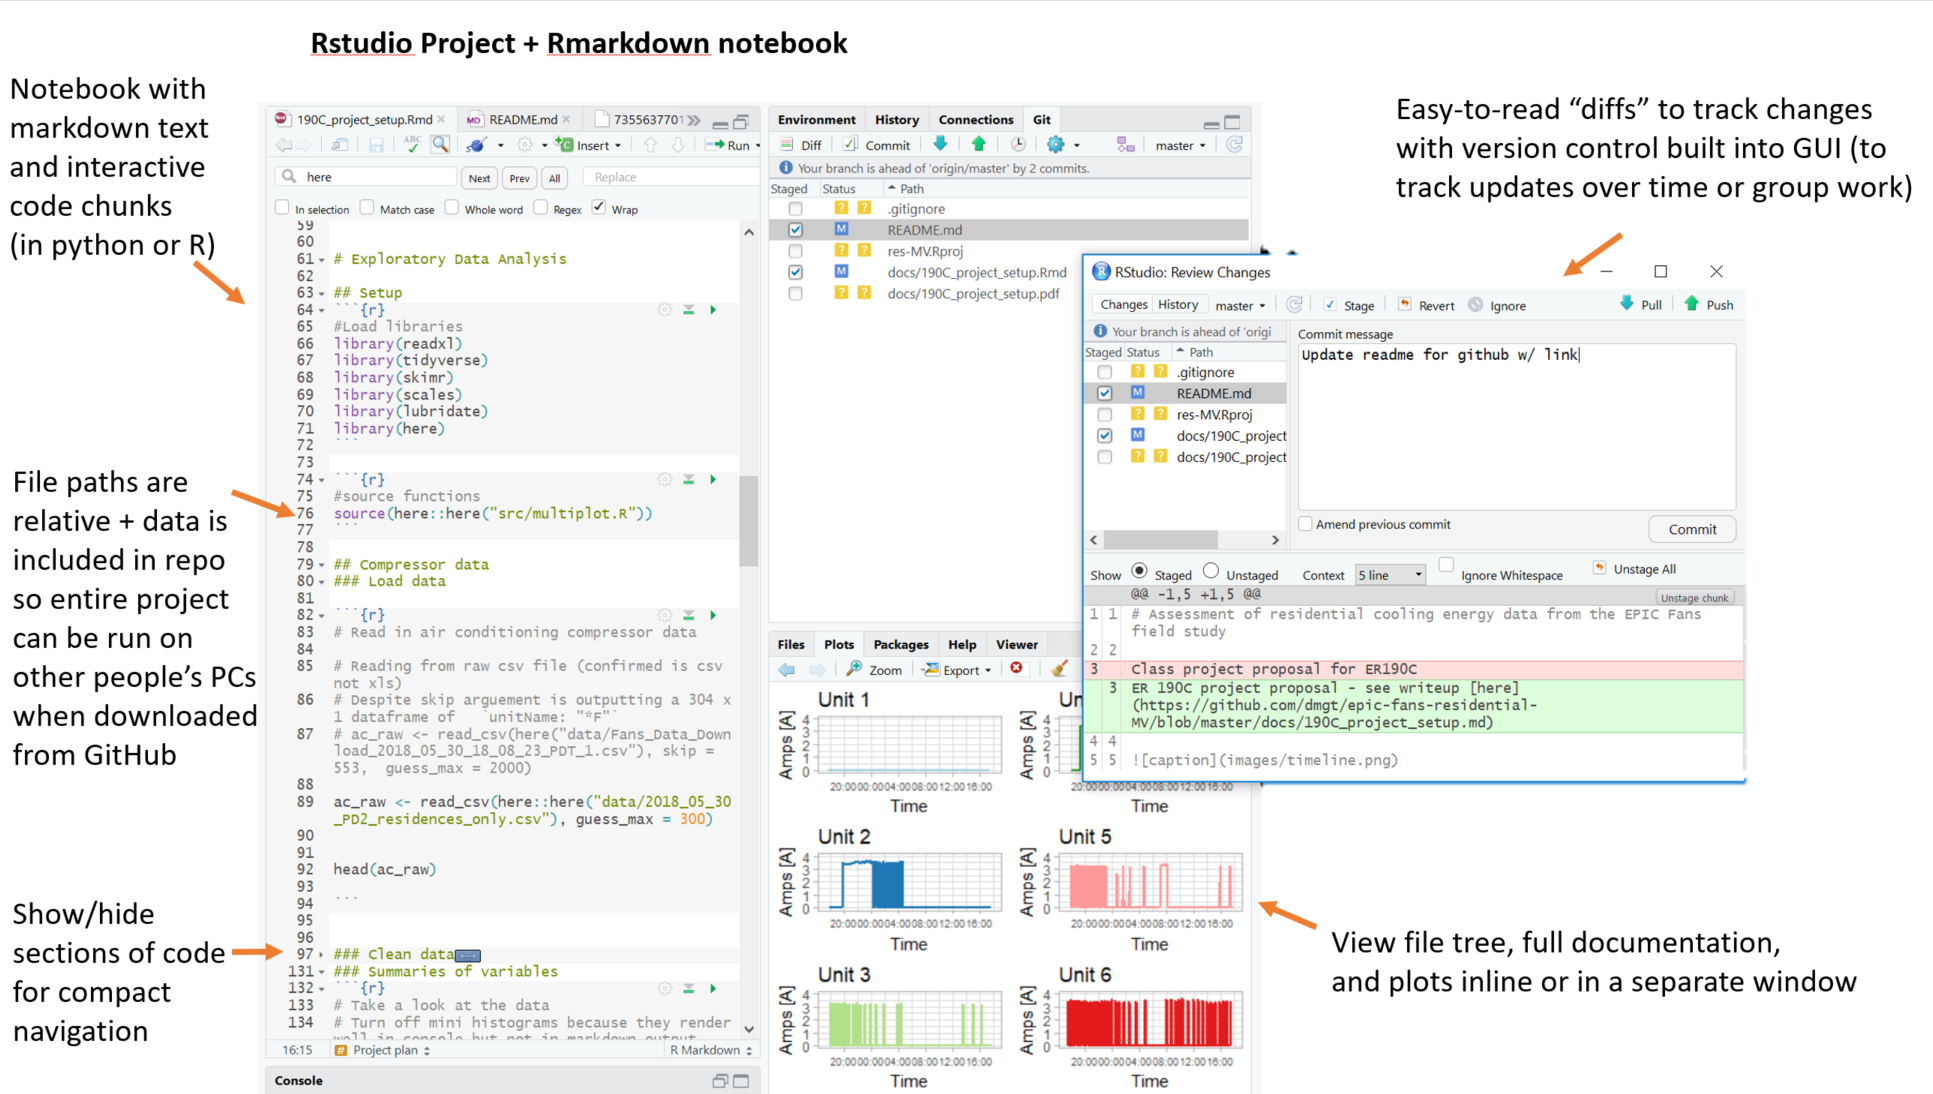
\includegraphics{C:/Users/Dana/3_Professional/CBE/Reproducibility/draft-template/Paper/SupplementaryMaterial/Figures/Rmd_notebook_example.png}

\pagebreak

\section{Introduction}\label{introduction}

\subsection{Benefits of air movement in
buildings}\label{benefits-of-air-movement-in-buildings}

Here is an example of an introductory paragraph with citations. The
following paragraph is from {[}1{]} :

\begin{quote}
Having the ability to increase the air speed in a room in a controlled
manner provides many advantages. It increases the heat transfer from
occupants to the environment by convection and evaporation, allowing
them to remain comfortable in warmer conditions {[}2--4{]}. Many
laboratory studies show that air movement provides comfort in warmer
conditions {[}5--8{]} even at 30°C and 80\% RH {[}9{]} and this is
accepted in existing thermal comfort standards (e.g. {[}10{]}). A field
study intervention adding ceiling fans to an air-conditioned office
found that occupants were equally or more comfortable at 26-27°C with
increased air movement than at 23°C without {[}11{]}. Giving occupants
control over air movement provides an instantaneous way to respond to
changing thermal comfort needs, responding faster than possible with
Heating Ventilation and Air Conditioning (HVAC) equipment designed to
condition the whole room {[}12{]}.
\end{quote}

\subsection{Terminology}\label{terminology}

Here is an example of a short terminology section, with terms quoted
from {[}1{]}.

\begin{itemize}
\tightlist
\item
  Fan rotational speed (\emph{N}): Physical fan rotational speed (rpm).
\item
  Fan airflow (\emph{Q}): Volumetric airflow rate through the fan blades
  (m³/s).
\item
  Blade height (\emph{H}): Distance from floor to blade, measured at hub
  (m).
\end{itemize}

\subsection{Another subtitle}\label{another-subtitle}

More text

\subsection{Objective}\label{objective}

This paper's primary goals are: (1) goal one; and (2) goal two

\section{Methods}\label{methods}

\subsection{Example data}\label{example-data}

The data in this template are is \texttt{iris} dataset freely avalible
at the \href{https://archive.ics.uci.edu/ml/datasets/iris}{University of
California Irvine Machine Learning Repository}, originally published by
R.A. Fischer in 1936. The dataset and its variables are described in the
included \texttt{iris-names} file under
\texttt{SupplementaryMaterial/Data} ). The \texttt{iris} dataset is also
avalible by default when you load R, but in this case we're reading it
in as a csv file to simulate working with external data.

\subsection{Another subtitle}\label{another-subtitle-1}

Here is an example of including a figure (which is included at the end
of the paper) Figure \ref{fig:experimentimage} is a saved .png image. It
appears that SVG images aren't recognized when markdown file is
converted to PDF.

Here is a footnote.\footnote{Example footnote.}

\begin{figure}
\centering
\includegraphics{C:/Users/Dana/3_Professional/CBE/Reproducibility/draft-template/Paper/SupplementaryMaterial/Figures/RLogo.png}
\caption{\label{fig:experimentimage}R logo, from
https://www.r-project.org/logo/, used under the terms of the Creative
Commons Attribution-ShareAlike 4.0 International license (CC-BY-SA 4.0)}
\end{figure}

\subsection{Another subtitle}\label{another-subtitle-2}

Here is another footnote and an example of programatically calculating a
number to be reported in the text\footnote{Another footnote.}. In the
next sentance, the number of iris classes is calculated from a short
piece of code, and the result is included as a variable, so that you
don't need to manually update the number in the text if more data is
added or the analysis changes. Figure \ref{fig:irises} shows each of the
3 iris classes in this experiment. The number for the figure refence in
the previous sentence is also being automatically generated based on its
order in the paper.

\begin{figure}
\centering
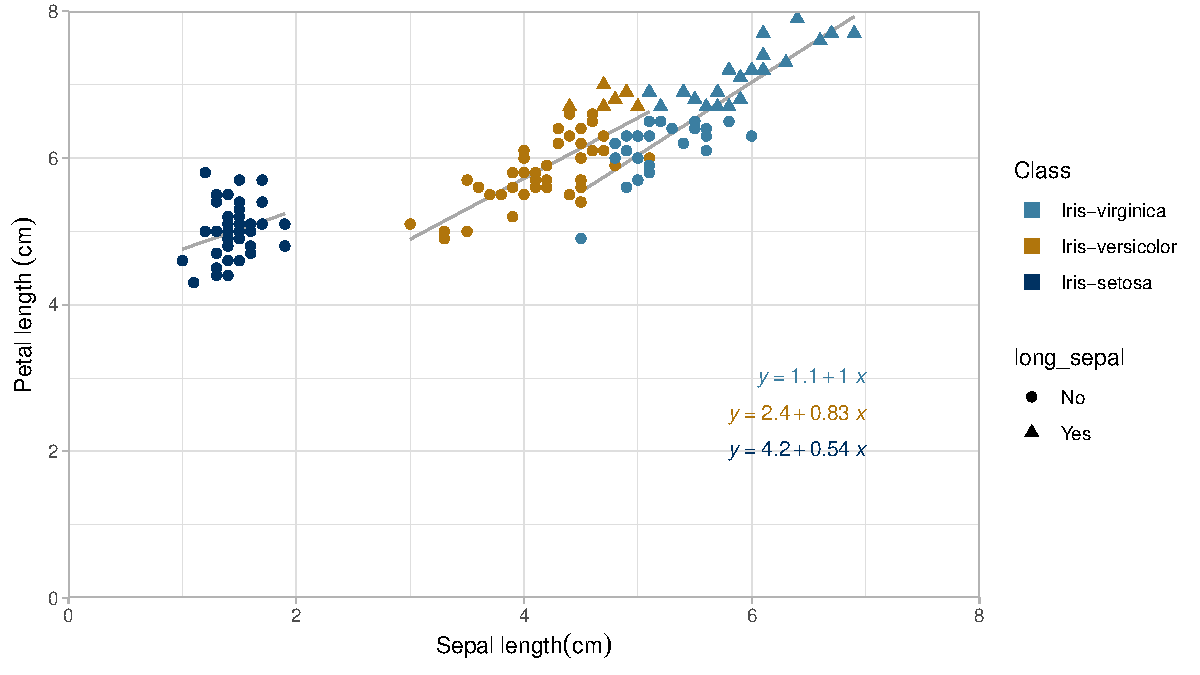
\includegraphics{Manuscript_files/figure-latex/irises-1.pdf}
\caption{\label{fig:irises}Petal and sepal lengths from iris dataset}
\end{figure}

\subsection{Reproducible research}\label{reproducible-research}

We wrote this paper using R Markdown. All of the text, references,
bibliography, data analysis and visualization occurs in one file
(Manuscript.Rmd), which automatically builds the document that we
submitted to the editor. The supplementary material contains the .Rmd
file as well as the entire measurement dataset.

\section{Results}\label{results}

\subsection{Subtitle}\label{subtitle}

Here is another example of using variables in the text that are directly
calculated from the underlying data. The median, lower and upper
quartiles of the \emph{versicolor} petal lengths are 4.35, 4, and 4.6 cm
respectively.

\subsection{Example of a violin plot}\label{example-of-a-violin-plot}

Figure \ref{fig:petalwidths} shows petal widths by iris type.

\begin{figure}
\centering
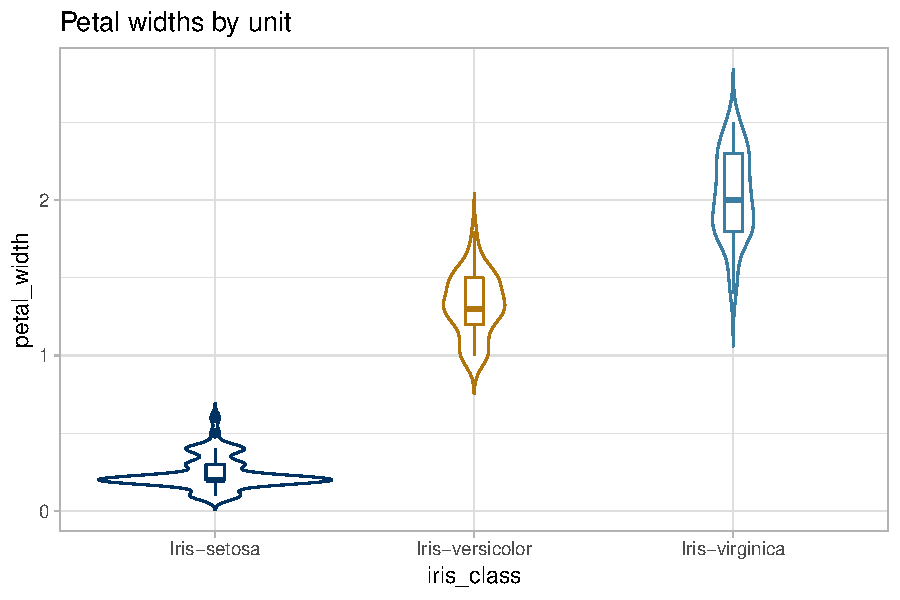
\includegraphics{Manuscript_files/figure-latex/petalwidths-1.pdf}
\caption{\label{fig:petalwidths}Petal widths by class}
\end{figure}

\subsubsection{Math example}\label{math-example}

Here is an example of an equation written using LATEX. The constants are
made up for this example :
\[AB_{avg} = 1 * \frac{\sqrt c}{D} - 0.23\ * \frac{E}{F}  = 45\] Here is
another equation:

\[ CD_{rated} = \frac{4*Q}{\pi*D^2} = 1.91~m/s\]

\subsection{Limitations}\label{limitations}

It is important to include a discussion of limitations in any paper.
Limitations of this template include:

\begin{itemize}
\tightlist
\item
  Figures are included after the txt, not at the location where they are
  discussed in the text
\item
  No example of a table yet
\end{itemize}

\section{Conclusions}\label{conclusions}

Text.

\section{Acknowledgements}\label{acknowledgements}

Agency (grant number 12345) supported this work, with cost share
provided by the Center for the Built Environment and Collaborating
Manufacturer. We thank Person1 and Person2 for setting up and acquiring
data for this experiment, and Person3 for preparing the first figure.

\section{Declaration of interest}\label{declaration-of-interest}

All authors declare no conflict of interest.

\section*{References}\label{references}
\addcontentsline{toc}{section}{References}

\hypertarget{refs}{}
\hypertarget{ref-rafteryDataCeilingFans}{}
{[}1{]} P. Raftery, Data for: Ceiling fans - Predicting indoor air
speeds based on full scale laboratory measurements, 1 (n.d.).
doi:\href{https://doi.org/10.17632/yk4jksgjdc.1}{10.17632/yk4jksgjdc.1}.

\hypertarget{ref-tanabeEstimationThermalSensation1993}{}
{[}2{]} S. Tanabe, Y. Hasebe, K.-i. Kimura, Y. Haga, Estimation of
thermal sensation using PMV and SET under high air movement conditions,
Journal of Thermal Biology. 18 (1993) 551--554.
doi:\href{https://doi.org/10.1016/0306-4565(93)90090-G}{10.1016/0306-4565(93)90090-G}.

\hypertarget{ref-tanabeEffectsAirTemperature1994a}{}
{[}3{]} S. Tanabe, K. ichi Kimura, Effects of air temperature, humidity,
and air movement on thermal comfort under hot and humid conditions, in:
ASHRAE Transactions, ASHRAE, 1994: pp. 953--969.

\hypertarget{ref-arensMovingAirComfort2009}{}
{[}4{]} E. Arens, S. Turner, H. Zhang, G. Paliaga, Moving air for
comfort, ASHRAE Journal. (2009).

\hypertarget{ref-rohlesEnhancingThermalComfort1982}{}
{[}5{]} F.H. Rohles, S.A. Konz, B.W. Jones, Enhancing Thermal Comfort
with Ceiling Fans, Proceedings of the Human Factors Society Annual
Meeting. 26 (1982) 118--120.
doi:\href{https://doi.org/10.1177/154193128202600203}{10.1177/154193128202600203}.

\hypertarget{ref-huangStudyDemandAir2013}{}
{[}6{]} L. Huang, Q. Ouyang, Y. Zhu, L. Jiang, A study about the demand
for air movement in warm environment, Building and Environment. 61
(2013) 27--33.
doi:\href{https://doi.org/10.1016/j.buildenv.2012.12.002}{10.1016/j.buildenv.2012.12.002}.

\hypertarget{ref-zhangReviewCorrectivePower2015a}{}
{[}7{]} H. Zhang, E. Arens, Y. Zhai, A review of the corrective power of
personal comfort systems in non-neutral ambient environments, Building
and Environment. 91 (2015) 15--41.
doi:\href{https://doi.org/10.1016/j.buildenv.2015.03.013}{10.1016/j.buildenv.2015.03.013}.

\hypertarget{ref-schiavonThermalComfortPerceived2017}{}
{[}8{]} S. Schiavon, B. Yang, Y. Donner, V.W.-C. Chang, W.W. Nazaroff,
Thermal comfort, perceived air quality, and cognitive performance when
personally controlled air movement is used by tropically acclimatized
persons, Indoor Air. 27 (2017) 690--702.
doi:\href{https://doi.org/10.1111/ina.12352}{10.1111/ina.12352}.

\hypertarget{ref-zhaiHumanComfortPerceived2015a}{}
{[}9{]} Y. Zhai, Y. Zhang, H. Zhang, W. Pasut, E. Arens, Q. Meng, Human
comfort and perceived air quality in warm and humid environments with
ceiling fans, Building and Environment. 90 (2015) 178--185.
doi:\href{https://doi.org/10.1016/j.buildenv.2015.04.003}{10.1016/j.buildenv.2015.04.003}.

\hypertarget{ref-ashraeASHRAEStandard552017}{}
{[}10{]} ASHRAE, ASHRAE Standard 55 - 2017 Thermal Environmental
Conditions for Human Occupancy, (2017).

\hypertarget{ref-lipczynskaThermalComfortSelfreported2018}{}
{[}11{]} A. Lipczynska, S. Schiavon, L.T. Graham, Thermal comfort and
self-reported productivity in an office with ceiling fans in the
tropics, Building and Environment. 135 (2018) 202--212.
doi:\href{https://doi.org/10.1016/j.buildenv.2018.03.013}{10.1016/j.buildenv.2018.03.013}.

\hypertarget{ref-kimOccupantComfortBehavior2019a}{}
{[}12{]} J. Kim, F. Bauman, P. Raftery, E. Arens, H. Zhang, G. Fierro,
et al., Occupant comfort and behavior: High-resolution data from a
6-month field study of personal comfort systems with 37 real office
workers, Building and Environment. 148 (2019) 348--360.
doi:\href{https://doi.org/10.1016/j.buildenv.2018.11.012}{10.1016/j.buildenv.2018.11.012}.

\end{document}


